%
%  untitled
%
%  Created by Dean Freestone on 2010-07-06.
%  Copyright (c) 2010 . All rights reserved.
%
\documentclass[]{article}

% Use utf-8 encoding for foreign characters
\usepackage[utf8]{inputenc}

% Setup for fullpage use
\usepackage{fullpage}

% Uncomment some of the following if you use the features
%
% Running Headers and footers
%\usepackage{fancyhdr}

% Multipart figures
%\usepackage{subfigure}

% More symbols

%\usepackage{latexsym}

% Surround parts of graphics with box
\usepackage{boxedminipage}

% Package for including code in the document
\usepackage{listings}

% If you want to generate a toc for each chapter (use with book)
\usepackage{minitoc}

% This is now the recommended way for checking for PDFLaTeX:
\usepackage{ifpdf}

\usepackage{amsmath,amssymb,amsfonts,epsfig} % Typical maths resource packages

%\newif\ifpdf
%\ifx\pdfoutput\undefined
%\pdffalse % we are not running PDFLaTeX
%\else
%\pdfoutput=1 % we are running PDFLaTeX
%\pdftrue
%\fi

\ifpdf
\usepackage[pdftex]{graphicx}
\else
\usepackage{graphicx}
\fi
\usepackage{color}
\newcommand{\dean}[1]{\textsf{\emph{\textbf{\textcolor{red}{#1}}}}} 


\title{Patient-Specific Neural Field Modeling from Micro-Electrode Data}
\author{In no specific order: Parham Aram, Dean R. Freestone, Kenneth Scerri, Michael Dewar,\\
 Andrew Zammit Mangion, Jacob A. Donoghue, Sydney S. Cash, Leigh R. Hochberg,\\
 David B. Grayden and Visakan Kadirkamanathan  }

\date{2010-07-06}

\begin{document}

\ifpdf
\DeclareGraphicsExtensions{.pdf, .jpg, .tif}
\else
\DeclareGraphicsExtensions{.eps, .jpg}
\fi

\maketitle


\begin{abstract}
	
	\begin{itemize}
		\item Background
		\item Method
		\item Result
		\item Conclusion
	\end{itemize}
\end{abstract}

\section{Introduction}
\begin{itemize}
	\item Understanding of macroscopic neurodynamics
	\item Neural field model
	\item Improvements in electrode technology with great spatiotemporal resolution
\end{itemize}
The aim of this paper is to great a patient-specific neural field model, by estimating parameters of a general mathematical model using data acquired from an epilepsy surgical candidate in a clinical setting. 
\section{Method}

\subsection{Neural Field Model}
The neural field equations used as the parametric form of the model are based on the influential papers from Wilson and Cowan~\cite{Wilson1973}, and Amari~\cite{Amari1977}. This class of model describes a continuous cortical sheet or surface, relating mean firing rates of pre and post-synaptic neural populations. The neural field, $v\left( {\mathbf{r},t} \right)$, at position $\mathbf{r}$ and time $t$, is the aggregated post-synaptic potentials described by the temporal convolution 
\begin{equation}
	\label{SpikesToPotential} v\left( {\mathbf{r},t} \right) = \int_{ - \infty }^t {h\left( {t - t'} \right)g\left( {\mathbf{r},t'} \right)dt'}, 
\end{equation}   
where $h(\cdot)$ is the synaptic response kernel and $g(\cdot)$ describes the mean firing rate. Assuming an infinite propagation velocity for action potentials within the field, the incoming firing rate the position $\mathbf{r}$ is described by spatial convolution
\begin{equation}
	\label{RateBasedInteractions} g\left( \mathbf{r},t \right) = \int_\Omega {w\left( \mathbf{r},\mathbf{r}' \right)f\left( v\left( \mathbf{r}',t \right) \right)\textrm{d}\mathbf{r}'}, 
\end{equation}
where $w(\cdot)$ is the spatial connectivity kernel and $\Omega$ is the spatial domain representing the cortical sheet or surface. The function $f(\cdot)$ relates mean post-synaptic potentials to mean firing rates and follows a sigmoid described by
\begin{equation}
	\label{ActivationFunction} f\left( v\left( \mathbf{r}', t \right) \right) = \frac{1}{1 + \exp \left( \varsigma \left( v_0 - v\left(\mathbf{r}',t\right) \right) \right)}, 
\end{equation}
where $v_0$ and $\varsigma$ describe the firing threshold the slope of the sigmoid respectively. By substituting equation~\ref{RateBasedInteractions} into equation~\ref{SpikesToPotential} we get the spatiotemporal model 
\begin{equation}
	\label{FullDoubleIntModel} v\left(\mathbf{r},t\right) =
	\int_{-\infty}^t 
	h\left(t - t'\right) \int_\Omega
	w\left(\mathbf{r},\mathbf{r}'\right) 
	f\left( v\left( \mathbf{r}',t' \right)\right)
	\textrm{d}\mathbf{r}'dt'.
\end{equation}
To arrive at the general integral-differential equation form of the model, we shall express the synaptic response kernel as a Green's function 
\begin{equation}
	\label{GreensFuncDef} Dh\left( t \right) = \delta \left( t \right), 
\end{equation}
where $D$ is a temporal differential operator and $\delta(t)$ is the Dirac-delta function giving 
\begin{equation}
	\label{eq:ContinuousWithOperator} 
	Dv\left( \mathbf{r},t \right) = \int_\Omega {w\left( \mathbf{r},\mathbf{r}' \right)f\left( {v\left( \mathbf{r}',t \right)} \right)\textrm{d}\mathbf{r}'}. 
\end{equation}
By assuming the synaptic response kernel is of first order has the form of
\begin{equation}
	\label{SynapticRespKernel} h(t) = \eta(t)\exp{\left(-\zeta t\right)}, 
\end{equation}
where $\zeta=\tau^{-1}$, $\tau$ is the synaptic time constant and $\eta(t)$ is the Heaviside step function, the operator $D$ is
\begin{equation}
	D=\frac{d}{dt} + \zeta,
\end{equation}
yielding
\begin{equation}
	\label{FinalFormContinuous} 
	\frac{dv\left( \mathbf{r},t \right)}{dt} + \zeta v\left( \mathbf{r},t \right) = \int_\Omega {w\left( \mathbf{r},\mathbf{r}' \right)f\left( {v\left( \mathbf{r}',t \right)} \right)\textrm{d}\mathbf{r}'}. 
\end{equation}
The neural field equations must be written as a discrete-time finite-dimensional model in order to relate it to patient-specific data. The discrete-time model is found applying the a first-order Euler method giving
\begin{equation}\label{EulerMethod}
	\frac{v\left( \mathbf{r},t+T_s \right)-v\left( \mathbf{r},t \right)}{T_s} + \zeta v\left(\mathbf{r},t \right) = \int_\Omega {w\left( \mathbf{r},\mathbf{r}' \right) f\left( {v\left( \mathbf{r}',t \right)}\right)\textrm{d}\mathbf{r}'},
\end{equation}
where $T_s$ is the time step or sampling period. To simplify the notation, the sample at the the current time step shall be indexed by $t$ and the future time step by $t+1$ for the rest of the paper. Rearranging equation~\ref{EulerMethod} gives the integro-difference equation (IDE) form
\begin{equation}
	\label{DiscreteTimeModel} 
	v_{t+1}\left(\mathbf{r}\right) = 
	\xi v_t\left(\mathbf{r}\right) + 
	T_s \int_\Omega { 
	    w\left(\mathbf{r},\mathbf{r}'\right)
	    f\left(v_t\left(\mathbf{r}'\right)\right) 
	\textrm{d}\mathbf{r}'}, 
\end{equation}
where $\xi = 1-T_s\zeta$. Finally, a disturbance term is added, to account for uncertainty and unmodelled inputs, to the IDE form giving
\begin{equation}
	\label{NoisyDiscreteTimeModel} 
	v_{t+1}\left(\mathbf{r}\right) = 
	\xi v_t\left(\mathbf{r}\right) + 
	T_s \int_\Omega { 
	    w\left(\mathbf{r},\mathbf{r}'\right)
	    f\left(v_t\left(\mathbf{r}'\right)\right) 
	\textrm{d}\mathbf{r}'} 
	+ e_t\left(\mathbf{r}\right), 
\end{equation}
where $e_t(\mathbf{r})$ is $i.i.d.$ such that $e_t(\mathbf{r})\sim\mathcal{GP}(\mathbf 0,\gamma(\mathbf{r}-\mathbf{r}'))$. Here $\mathcal{GP}(\mathbf 0,\gamma(\mathbf{r}-\mathbf{r}'))$ denotes a zero mean spatial Gaussian process with covariance function $\gamma(\mathbf{r}-\mathbf{r}')$~\cite{Rasmussen2005}.
To reduce the model to a finite-dimensional system the neural field is approximated by a basis function decomposition where
\begin{equation}
	\label{DefFieldDecomp} v_t\left(\mathbf{r}\right) \approx \boldsymbol{\phi}^{\top}\left(\mathbf{r}\right) \mathbf{x}_t 
\end{equation}
and $\mathbf{x}_t$ is a state vector that weights a vector of two-dimension Gaussian basis functions, $\boldsymbol{\phi}(\mathbf{r})$, described by
\begin{equation}\label{eq:FieldBasisFunction}
	\boldsymbol\phi\left(\mathbf{r}-\mathbf{r}'\right) =
\exp{\left(-\frac{(\mathbf{r}-\mathbf{r}')^\top(\mathbf{r}-\mathbf{r}')}{\sigma_{\phi}^2}\right)}. 
\end{equation}
The parameter $\sigma_{\phi}$ controls the basis function width and is inferred by frequency analysis. Substituting equation~\ref{DefFieldDecomp} into~\ref{NoisyDiscreteTimeModel} gives to approximate model
\begin{equation}
	\label{eq:reduced continuous model}
	\boldsymbol{\phi}^{\top}(\mathbf{r})\mathbf{x}_{t+1}= T_s\int_\Omega{f(\boldsymbol{\phi}^{\top}(\mathbf{r}')\mathbf{x}_t )w(\mathbf{r},\mathbf{r}')\textrm{d}\mathbf{r}'}
	+ \xi\boldsymbol{\phi}^{\top}(\mathbf{r})x_t + e_t(\mathbf{r}). 
\end{equation}
Next we multiply equation~\ref{eq:reduced continuous model} by $\boldsymbol{\phi}(\mathbf{r})$ and integrate over the spatial domain, $\Omega$, to get 
\begin{equation}
	\label{StartofReduction}
 	\int_\Omega {\boldsymbol{\phi} \left(\mathbf{r}\right)\boldsymbol{\phi}^{\top}\left(\mathbf{r}\right) \textrm{d}\mathbf{r}} \mathbf{x}_{t+1} = T_s \int_\Omega {\boldsymbol{\phi} (\mathbf{r}) \int_\Omega {w(\mathbf{r},\mathbf{r}') f(\boldsymbol{\phi}^{\top}(\mathbf{r}') \mathbf{x}_t ) \textrm{d}\mathbf{r}'}\textrm{d}\mathbf{r}} + \xi\int_\Omega{\boldsymbol{\phi}(\mathbf{r})\boldsymbol{\phi}^{\top}(\mathbf{r})\textrm{d}\mathbf{r}} \mathbf{x}_t + \int_\Omega{\boldsymbol{\phi} (\mathbf{r}) e_t(\mathbf{r})\textrm{d}\mathbf{r}}. 
\end{equation}
Now by defining the matrix
\begin{equation}\label{eq:DefGamma}
	\boldsymbol{\Gamma} \triangleq \int_\Omega {\boldsymbol{\phi} \left(\mathbf{r}\right)\boldsymbol{\phi} ^{\top}\left(\mathbf{r}\right)\textrm{d}\mathbf{r}} 
\end{equation}
enables the pseudo inverse of $\boldsymbol{\phi(\mathbf{r})}$ to be taken, such that the state vector can is isolated on the left-hand-side as
\begin{equation}\label{eq:ReducedForm}
	 \mathbf{x}_{t+1} = T_s\boldsymbol{\Gamma}^{-1}
	 \int_\Omega \boldsymbol{\phi}(\mathbf{r}) 
	 \int_\Omega w(\mathbf{r},\mathbf{r}')f(\boldsymbol{\phi}^{\top}(\mathbf{r}')\mathbf{x}_t) \textrm{d}\mathbf{r}' \textrm{d}\mathbf{r} 
	 + \xi\mathbf{x}_t + \boldsymbol{\Gamma}^{-1} \int_\Omega{\boldsymbol{\phi}(\mathbf{r}) e_t(\mathbf{r})\textrm{d}\mathbf{r}}.
\end{equation}
A property of the basis function decomposition it the preservation of the Gaussianality of the disturbance term. The decomposition disturbance term is defined as
\begin{equation}\label{eq:Wt} 
	\mathbf{e}_t \triangleq \boldsymbol{\Gamma}^{-1}\int_\Omega {\boldsymbol{\phi} ( \mathbf{r} )e_t( \mathbf{r} )\textrm{d}\mathbf{r}},
\end{equation}
where $\mathbf{e}_t \sim\mathcal{N}(\mathbf 0,\boldsymbol\Sigma_e)$. The covariance matrix is defined as (see the Supporting Information, S1, for the derivation)
\begin{equation}
	\boldsymbol\Sigma_e \triangleq \mathbf{\Gamma}^{-1}\int_{\Omega}\int_{\Omega}\boldsymbol{\phi}\left(\mathbf r\right) \gamma\left(\mathbf r- \mathbf r' \right)\boldsymbol{\phi}\left(\mathbf r'\right)^{\top}d\mathbf r' d\mathbf r\mathbf{\Gamma}^{- \top}. 
\end{equation}

To relate the model to the data the electrodes are also modelled. The electrodes have a pick-up range (for LFPs) of approximately 400~$\mu$m. Therefore, we model the electrodes as a spatial convolution of a Gaussian shaped sensor kernel (using a width parameters of 400~$\mu$m) with the neural field. The observation equation is
\begin{equation}
    \label{eq:ObservationEquation}
	\mathbf{y}_t =
	\int_{\Omega}{
	    m\left(\mathbf{r}_n-\mathbf{r}'\right)v_t\left(\mathbf{r}'\right)
	\textrm{d}\mathbf{r}'} + 
	\boldsymbol{\varepsilon}_t, 
\end{equation}
where $\mathbf{r}_n$ defines the location of the sensors in the field, $n=1,...,N$ indexes the sensors and $\boldsymbol{\varepsilon}_t \sim \mathcal{N}\left(0,\boldsymbol{\Sigma}_{\varepsilon}\right)$. $\mathcal{N}\left(0,\boldsymbol{\Sigma}_{\varepsilon}\right)$ denotes the multivariate normal distribution with mean zero and covariance matrix $\boldsymbol{\Sigma}_{\varepsilon}$. The sensor kernel, $m(\mathbf{r}-\mathbf{r}')$, is defined by 
\begin{equation}
	m\left(\mathbf{r}-\mathbf{r}'\right) = \exp{\left(-\frac{(\mathbf{r}-\mathbf{r}')^\top(\mathbf{r}-\mathbf{r}')}{\sigma_m^2}\right)},
\end{equation}
where $\sigma_m$ sets the sensor width. Under the assumption that the basis function decomposition is accurate, the observation equation of the reduced model is found by substituting equation~\ref{DefFieldDecomp} into~\ref{eq:ObservationEquation} giving
\begin{equation}\label{eq:ReducedObservationEquation}
	\mathbf{y}_t = \int_{\Omega}{m\left(\mathbf{r}_n-\mathbf{r}'\right)\boldsymbol{\phi}^{\top}\left(\mathbf{r'}\right) \mathbf{x}_t\textrm{d}\mathbf{r}'} + \boldsymbol{\varepsilon}_t. 
\end{equation}
The observation equation is linear with respect to the state and can be written in the more compact form
\begin{equation}\label{ObservationEquation} 
	\mathbf{y}_t = \mathbf{C}\mathbf{x}_t + \boldsymbol{\varepsilon}_t,
\end{equation}
where the observation matrix is 
\begin{equation}
	\mathbf{C} = \left[
	\begin{array}{{ccc}} 
		c_{1,1} & \dots & c_{1,L} \\
		\vdots & \ddots & \vdots \\
		c_{N,1} & \dots & c_{N,L} 
	\end{array}
	\right] 
\end{equation}
and 
\begin{equation}
	c_{i,j} = \int_{\Omega}m(\mathbf{r}_i - \mathbf{r}')\boldsymbol{\phi}_j(\mathbf{r}')\textrm{d}\mathbf{r}'. 
\end{equation}

\dean{I will do the connectivity kernel decomposition bit after the correlation analysis, because we can use it to say something about heterogeneity and isotropy.}

\subsection{Data Collection and Pre-processing}

Data was collected from a patient undergoing work-up for surgical resection of epileptic brain tissue. The standard procedure for the resective surgery involves implantation of subdural electrodes for intracranial EEG monitoring (iEEG). Data from these electrodes provide information for mapping functional and pathological tissue to define the surgical margins. In addition to standard iEEG electrodes, data was collected in parallel from a Neuroport system (Blackrock microsystems, Utah, USA) incorporating a micro-electrode array. This data was collected with informed consent from the patient under ethics approval from the MGH human research ethics committee..?? Figure~\ref{MRI_CT} shows the position of the iEEGs electrodes and the micro-electrode array. The iEEG electrode covers the temporal lobe, and the micro-electrode placement was targeted at.. The micro-electrode array consisted of square grid of 96 (10 by 10 with the corner electrodes missing). The x,y electrode spacing was 400~$\mu m$, yielding a coverage of 4 by 4~mm. Data from the Neuroport system was acquired with a sampling rate of 30~kHz, with hardware filters in the range of~\dean{??}. 

During the time-course of the iEEG monitoring period, several seizures were recorded. This study focuses on the local field potential (LFP) data recorded with the micro-electrode during a seizure. 

The first pre-processing step was to identify channels that had very poor signal quality. These channels were set to the $nan$ data type. Following this, the data was re-referenced to a common average montage to remove common mode artifact and the effect of the reference electrode. Next the data was low-pass filtered with a cut-off frequency of 100~Hz. The data was then resampled from 30~kHz to 5~kHz. To enable spatial visualisation and spatial frequency analysis, the corrupted channels that were set to $nan$, were interpolated using data from all neighbouring channels.

\subsection{Spatiotemporal Data Analysis}
The first 8 channels of the LFP time series from the seizure is shown in Figure~\ref{fig:TimeSeries}. For the analysis, the time series was segmented into three periods; the pre-seizure period, seizure period and post-seizure period. The seizure onset is marked by the red dotted line and the seizure end is marked by the blue dashed line. 

An example to illustrate the spatial aspects of the observed neural field is shown in Figure~\ref{fig:FieldObserations}. Each subplot in the figure shows the observed field at a sample of the pre-processed data, with each plot separated in time by 2.5~ms. The figure shows spatially correlated activity.

The spectral properties of the recorded time series for each of the time segments are shown in Figure~\ref{fig:TemporalFreqObservation}. Each plot shows the averaged (across channels) spectrum of the data. The pre-seizure period shows a decay in power at a typical $1/f^2$ rate. The seizure period has higher power at low and high ends of the spectrum. In addition, there is a peak in the power of the LFPs at ~51~Hz during the seizure. This peak would be difficult to observe in European, Asian and other countries due to the 50~Hz mains power frequency. The post-seizure period shows a large increase in lower frequency power...

Figure~\ref{fig:SpatialFreqObservation} shows the results of spatial frequency analysis of the observed neural field. Throughout this paper the spatial frequency shall be denoted by $\nu$. Each subplot is the average (across time) spatial frequency during either the pre-seizure, seizure or post-seizure periods. The spatial frequency of the neural field is governed by disturbances (inputs from outside the field) and the underlying connectivity structure. The symmetry in the plots provides some evidence for homogeneous and isotropic connectivity.   

Figure~\ref{fig:DiagSpatialFreqObservation} shows diagonal cross-sections of the spatial frequency plots. From this figure we can see that the spatial cut-off frequency (-3~dB point) is $\nu_c \approx 0.26$~Hz. The profile of the diagonal cross-section indicates that the field is adequately sampled from the micro-electrode array, where the power drops by approximately 25~dB at the maximum observable spatial frequency (according to Shannon's sampling theorem) indicating spatial aliasing will have an insignificant effect on the sampled data. The spatial cut-off frequency provides information on the complexity of the model required to represent the neural field. Considering the field is band-limited, we can represent it by a finite set of continuous basis functions. According the Shannon's sampling theorem, the minimum spacing between basis functions, $\Delta_{\phi}$, to describe the field is
\begin{equation}\label{eq:BasisFunctionSeparation}
	\Delta_{\phi} \leq \frac{1}{2\rho_{\phi}\boldsymbol{\nu}_{c}}
\end{equation}
where $\rho_{\phi} \in \mathbb{R} \ge 1$ is an oversampling parameter to determine the basis function separation.

\subsection{Estimating Support For Connectivity Kernel}
Under the assumption that the sensors are not spatially band-limiting the spectral content of the field and the connectivity kernel is homogeneous, the support for the connectivity kernel can be inferred by studying the spatial cross-correlation between consecutive observations. The deterministic component of the spatial mapping between consecutive fields is due to the convolution of the connectivity kernel with the firing rates. Although the relationship between the field and the firing rate is nonlinear, the cross-correlation analysis still extracts meaningful results. This can be seen by considering the three operating regions of the sigmoid. When the mean membrane voltage is below the active region of the sigmoid, the firing rate will be approximately zero and only very small spatial correlations will observed. Therefore, this will not contribute to the results. Within the active region the sigmoid can be approximated by a linear function between consecutive samples, given a sufficiently high sampling rate. Therefore, linear cross-correlation analysis is appropriate. When the sigmoid is in the saturated region, the correlation coefficients will be higher, but not provide a meaningful measure of the kernel weight or gain. Therefore, we can not estimate the gain for the kernel using cross-correlation analysis, but the spatial extent can still be inferred. The gain for the kernel will be inferred using the EM algorithm described below.

Figure~\ref{fig:SpatialCrossCorrelation} shows the average (across time) cross-correlations between consecutive field observations for the different time periods of the seizure progression. By averaging over time, the effect of the disturbance is reduced allowing for the support of the kernel to be seen. The subplots of the figure show that the connectivity kernel exhibits local excitation with surround inhibition. The plots indicate the support for excitatory aspect of the kernel centred at the origin is -2~mm to 2~mm in the $x$ direction and slightly wider in the $y$ direction. Although the kernel is not isotropic, we will approximate it as being isotropic. This is for computation reasons.

The assumption of homogeneity was tested by performing the cross-correlation analysis on 4 equal sized subsections of the field observations. The subsections consisted $6\times6$ electrode grids, such that they overlapped by one electrode row and column. The overlap was required so the subsections where large enough for the support of the kernel to be seen in the cross-correlation analysis. The results of the analysis can be seen in Figure~\ref{fig:HomogeneityTest}. The results show that each subsection of the field has similar cross-correlations, with each subplot showing local excitation with surround inhibition. From this analysis, we will approximate the connectivity kernel as being homogeneous.

\subsection{Parametrisation of Connectivity Kernel}
The connectivity kernel can be decomposed as 
\begin{equation}\label{eq:DefKernelDecomp}
	 w\left(\mathbf{r},\mathbf{r}'\right) \approx \boldsymbol{\psi}^\top\left(\mathbf{r},\mathbf{r}'\right) \boldsymbol{\theta},
\end{equation}
where $\boldsymbol{\psi}(\mathbf{r},\mathbf{r}')$ is a vector of Gaussian basis functions and $\boldsymbol{\theta}$ is a vector of scaling parameters. By assuming a Gaussian isotropic connectivity structure, the kernel basis functions can be written as $\boldsymbol{\psi}(\mathbf{r}-\mathbf{r}')$. We will assume that we know the parametric form of the connectivity basis functions from the correlation analysis, where the scaling parameters $\boldsymbol{\theta}$ are unknown.
Substituting equation~\ref{eq:DefKernelDecomp} into equation\ref{eq:ReducedForm} gives
\begin{equation}\label{eq:KernelDecompForm}
	 \mathbf{x}_{t+1} = T_s\boldsymbol{\Gamma}^{-1}
	 \int_\Omega \boldsymbol{\phi}(\mathbf{r}) 
	 \int_\Omega \boldsymbol{\psi}^\top\left(\mathbf{r},\mathbf{r}'\right) \boldsymbol{\theta} f(\boldsymbol{\phi}^{\top} (\mathbf{r}')\mathbf{x}_t) \textrm{d}\mathbf{r}' \textrm{d}\mathbf{r} 
	 + \xi\mathbf{x}_t + \mathbf{e}_t(\mathbf{r}).
\end{equation}
The connectivity kernel weights can be shifted outside the integral giving
\begin{equation}
	 \mathbf{x}_{t+1} = T_s\boldsymbol{\Gamma}^{-1}
	 \int_\Omega \boldsymbol{\phi}(\mathbf{r}) 
	 \int_\Omega \boldsymbol{\psi}^{\top} (\mathbf{r}-\mathbf{r}')f(\boldsymbol{\phi}^{\top}(\mathbf{r}')\mathbf{x}_t) \textrm{d}\mathbf{r}' \textrm{d}\mathbf{r} \boldsymbol{\theta}  
	 + \xi\mathbf{x}_t + \mathbf{e}_t(\mathbf{r}).
\end{equation}
Now taking the basis function vector inside the inner integrand gives
\begin{equation}\label{eq:ReucedFormWithKernelDecomp}
	 \mathbf{x}_{t+1} = T_s\boldsymbol{\Gamma}^{-1}
	 \int_\Omega \int_\Omega \boldsymbol{\phi}(\mathbf{r})\boldsymbol{\psi}^{\top} (\mathbf{r}-\mathbf{r}')f(\boldsymbol{\phi}^{\top}(\mathbf{r}')\mathbf{x}_t) \textrm{d}\mathbf{r}' \textrm{d}\mathbf{r} \boldsymbol{\theta}  
	 + \xi\mathbf{x}_t + \mathbf{e}_t(\mathbf{r}).
\end{equation}
This equation can be simplified by exploiting the isotropy of the kernel and, hence, the basis functions used to represent it where
\begin{equation}
	\boldsymbol{\psi} (\mathbf{r}-\mathbf{r}') = \boldsymbol{\psi} (\mathbf{r}'-\mathbf{r}).
\end{equation}
To make the simplification, we define
\begin{equation}\label{eq:DefPsi}
	\boldsymbol{\Psi}(\mathbf{r}') \triangleq T_s\boldsymbol{\Gamma}^{-1}\int_\Omega {\boldsymbol{\phi}(\mathbf{r})\boldsymbol{\psi}^{\top} (\mathbf{r}'-\mathbf{r})\textrm{d}\mathbf{r}},
\end{equation}
which is a constant $L \times n_{\theta}$ matrix that is defined analytically, where $L$ is the number of basis functions (and states) and $n_{\theta}$ is the number of connectivity kernel basis functions. Substituting equation~\ref{eq:DefPsi} into~\ref{eq:ReucedFormWithKernelDecomp} gives
\begin{equation}
	\mathbf{x}_{t+1} = \int_\Omega \boldsymbol{\Psi}(\mathbf{r}') f(\boldsymbol{\phi}^{\top}(\mathbf{r}')\mathbf{x}_t) \textrm{d}\mathbf{r}' \boldsymbol{\theta} + \xi\mathbf{x}_t 
+ \mathbf{e}_t(\mathbf{r}).
\end{equation}
This substitution exploits the isotropy of the connectivity kernel basis functions, allowing us to swap the convolution in equation~\ref{eq:ReucedFormWithKernelDecomp}, which is computationally demanding, with the convolution in equation~\ref{eq:DefPsi}. This provides a dramatic increase in estimation speed, since the matrix $\boldsymbol\Psi(\mathbf{r}')$ can be calculated analytically. This is of great importance as it lowers the computational demands of the estimation algorithm.

As a result of the model reduction via the basis function decomposition and the decomposition of the connectivity kernel the state space model is formed
\begin{align}
 \mathbf x_{t+1}&=q(\mathbf x_t)\boldsymbol\theta+\xi \mathbf x_t+\boldsymbol e_t(\mathbf r) \\
 \mathbf y_t&=\mathbf C \mathbf x_t+\boldsymbol \epsilon_t,
\end{align}
where the nonlinear function, $q(\cdot)$, is defined as
\begin{equation}\label{eq:QmatrixForSigmapoints}
	q(\mathbf{x}_t) = \int_\Omega \boldsymbol{\Psi}(\mathbf{r}') f(\boldsymbol{\phi}^{\top}(\mathbf{r}')\mathbf{x}_t) d\mathbf{r}'.
\end{equation}
\section{Estimation Algorithm}

\subsection{E-Step}
The unscented Rauch-Tung-Striebel smoother (URTSS)~\cite{Sarkka2010} was used for the state estimation. The URTSS incorporates an unscented Kalman filter (UKF)~\cite{Julier1997, Merwe2003} in a forward step to estimate posterior states, $\hat{\mathbf x}_t^{f}$, followed by a backward step to compute the smoothed state estimates, $\hat{\mathbf x}_t^{b}$. The first and second order moments of the predicted state are captured by propagating the so-called sigma points through the state equation. An additional element to the URTSS algorithm was created to approximate $q(\mathbf{x}_t)$, which is required for the M-step. 

This is accomplished by taking the first-order truncated Taylor-series expansion of $q(\mathbf x_t)$ around the mean of the state at each time instant for the sigmoidal activation function, i.e.
\begin{equation}\label{eq:SigmoidTaylor}
 f(\boldsymbol \phi^\top(\mathbf r')\mathbf x_t) \approx f(\boldsymbol \phi^\top(\mathbf r')\mathbf {\hat x}_t)+  \boldsymbol \phi^\top(\mathbf r')(\mathbf x_t - \mathbf  {\hat x}_t)f'(\boldsymbol \phi^\top(\mathbf r')\mathbf {\hat x}_t)
\end{equation}
where 
\begin{equation}\label{eq:SigmoidDerivative}
 f'(\boldsymbol \phi^\top(\mathbf r')\mathbf {x}_t)=\varsigma f(\boldsymbol \phi^\top(\mathbf r')\mathbf {x}_t)\left( 1-\frac{f( \boldsymbol \phi^\top(\mathbf r')\mathbf {x}_t)}{f_{max}}\right)
\end{equation}
substituting \ref{eq:SigmoidTaylor} in \ref{eq:QmatrixForSigmapoints}  we get an approximation for $q(\mathbf x_t)$ as
\begin{equation}\label{eq:qTaylor}
 q(\mathbf x_t) \approx q(\mathbf {\hat x}_t)+\int_\Omega \boldsymbol{\Psi}(\mathbf{r}')\boldsymbol \phi^\top(\mathbf r') (\mathbf x_t - \mathbf  {\hat x}_t)f'(\boldsymbol \phi^\top(\mathbf r')\mathbf {\hat x}_t) d\mathbf{r}'
\end{equation}

The algorithm for the modified URTSS can be seen in Table~\ref{tab:URTSSAlgorithm}.

\subsection{M-Step}


\subsection{$\mathcal Q$-function}
The goal of the M-step is to maximise the likelihood function $p(\mathbf Y;\boldsymbol \theta,\xi)$ given the joint distribution $p(\mathbf X,\mathbf Y;\boldsymbol \theta,\xi)$ over the observed variables $\mathbf Y$ and hidden variables $\mathbf X$ that is governed by parameters $\boldsymbol \theta$ and $\xi$. Unfortunately, it is often not possible to maximise the likelihood $p(\mathbf Y;\boldsymbol \theta,\xi)$ directly. However, by using the relationship between $p(\mathbf Y;\boldsymbol \theta,\xi)$ and $p(\mathbf X,\mathbf Y;\boldsymbol \theta,\xi)$ it is possible to compute a sequence of parameter estimates that converges on the maximum likelihood parameter estimate. 

Expanding the joint distribution $p(\mathbf X,\mathbf Y;\boldsymbol \theta,\xi)$ we have
\begin{equation}\label{eq:jointdistribution}
 p(\mathbf X,\mathbf Y;\boldsymbol \theta,\xi)=\prod_{t=0}^{T-1} p(\mathbf y_{t+1}|\mathbf x_{t+1})p(\mathbf x_{t+1}|\mathbf x_{t};\boldsymbol \theta, \xi)p(\mathbf x_0).
\end{equation}
The $\mathcal Q$-function, or lower-bound on the likelihood, can be written in terms of joint distribution components as
\begin{align}
 \mathcal Q(\boldsymbol \theta,\xi,\boldsymbol\theta',\xi')&=\mathbf E_{\boldsymbol (\theta',\xi')}\left[\ln p(\mathbf X,\mathbf Y;\boldsymbol \theta,\xi)\right] \\
&=\mathbf E_{\boldsymbol (\theta',\xi')}\left[\sum_{t=0}^{T-1}\ln p(\mathbf y_t|\mathbf x_t)+\sum_{t=0}^{T-1}\ln p(\mathbf x_t|\mathbf x_{t-1};\boldsymbol \theta, \xi)+\sum_{t=0}^{T-1}\ln p(\mathbf x_0)\right],
\end{align}
where $ \mathbf E_{\boldsymbol (\theta',\xi')}$ denotes expectation taken with respect to the distribution $p(\mathbf X | \mathbf Y;\boldsymbol \theta',\xi') $ where $\boldsymbol \theta'$ and $\xi'$are the current parameter estimates. It should be noted that
$p(\mathbf y_t|\mathbf x_t)$ and $p(\mathbf x_0)$ are not functions of parameter set and therefore $\mathcal Q$-function can be rewritten as
\begin{equation}
\mathcal Q(\boldsymbol \theta,\xi,\boldsymbol\theta',\xi')=\mathbf E_{(\theta',\xi')}\left[\sum_{t=0}^{T-1}\ln p(\mathbf x_t|\mathbf x_{t-1};\boldsymbol \theta ,\xi)\right]+\mathrm{const}
\end{equation}
the constant term can be ignored since it is not affecting the derivative with respect to the parameters. 
The Gaussian distribution of the disturbance, $e_t(\mathbf r)\sim \mathcal N(\mathbf 0,\boldsymbol\Sigma_e(\mathbf r,\mathbf r'))$ results into the following conditional distribution of the state at $t+1$
\begin{equation}
 p(\mathbf x_{t+1} | \mathbf x_t;\boldsymbol\theta,\xi)=\alpha e^{-(\mathbf x_{t+1}-q(\mathbf  x_t)\boldsymbol\theta-\xi  \mathbf x_t)^\top\boldsymbol\Sigma_e^{-1}(\mathbf x_{t+1}-q( \mathbf x_t)\boldsymbol\theta-\xi \mathbf  x_t)}
\end{equation}
where $\alpha$ is the normalising constant. By expanding the exponent and taking $\log$ we get
\begin{eqnarray}\label{eq:Qfunction}
  \ln p(\mathbf x_{t+1} | \mathbf x_t;\boldsymbol\theta,\xi)&=&\ln \alpha-\mathbf x_{t+1}^\top\boldsymbol\Sigma_e^{-1}\mathbf x_{t+1}+2\mathbf x_{t+1}^\top\boldsymbol\Sigma_e^{-1}q( \mathbf x_t)\boldsymbol\theta+2\xi \mathbf x_{t+1}^\top\boldsymbol\Sigma_e^{-1}\mathbf x_t\nonumber \\
&&-\boldsymbol\theta^\top q^\top(\mathbf x_t)\boldsymbol\Sigma_e^{-1}q(\mathbf x_t)\boldsymbol\theta-2\xi \mathbf x_t^\top\boldsymbol\Sigma_e^{-1}q(\mathbf x_t)\boldsymbol\theta-\xi^2\mathbf x_t^\top\boldsymbol\Sigma_e^{-1}\mathbf x_t.
\end{eqnarray}
Taking trace and rearranging, using the invariant cyclic permutations property of the trace, this distribution can be written as
\begin{eqnarray}\label{eq:Qfunctionintrace}
  \ln p(\mathbf x_{t+1} | \mathbf x_t;\boldsymbol\theta,\xi)&=&\ln \alpha-\mathbf x_{t+1}^\top\boldsymbol\Sigma_e^{-1}\mathbf x_{t+1}+2\mathbf x_{t+1}^\top\boldsymbol\Sigma_e^{-1}q( \mathbf x_t)\boldsymbol\theta+2\xi \mathrm{tr} \left\lbrace \mathbf x_t\mathbf x_{t+1}^\top\boldsymbol\Sigma_e^{-1}\right\rbrace \nonumber \\
&&-\boldsymbol\theta^\top q^\top(\mathbf x_t)\boldsymbol\Sigma_e^{-1}q(\mathbf x_t)\boldsymbol\theta-2\xi \mathbf x_t^\top\boldsymbol\Sigma_e^{-1}q(\mathbf x_t)\boldsymbol\theta-\xi^2\mathrm{tr}\left\lbrace \mathbf x_t \mathbf x_t^\top\boldsymbol\Sigma_e^{-1}\right\rbrace. 
\end{eqnarray}
Now taking the expectation of the log likelihood function for all time instants gives the $\mathcal Q$-function, which is the lower-bound that needs to be maximised to gain optimal parameter estimates. The $\mathcal Q$-function is written as  
\begin{align}\label{eq:Voldermont}
 \mathcal Q(\boldsymbol \theta,\xi,\boldsymbol\theta',\xi')&=\beta+2\Xi_0\boldsymbol\theta+
2\xi tr\left\lbrace \Xi_1 \boldsymbol\Sigma_e^{-1}\right\rbrace \nonumber \\
&-\boldsymbol\theta^\top \Xi_2\boldsymbol\theta-2\xi \Xi_3 \boldsymbol\theta - \xi^2 tr \left\lbrace\Xi_4\boldsymbol\Sigma_e^{-1} \right\rbrace \tag{Voldermont}
\end{align}
where 
\begin{align}
	\beta &= \sum_{t=0}^{T-1}\mathbf E_{(\theta',\xi')}\left[ \ln \alpha-\mathbf x_{t+1}^\top\boldsymbol\Sigma_w^{-1}\mathbf x_{t+1}\right] \label{eq:def of beta} \\
\Xi_0&=\sum_{t=0}^{T-1}\left[ \mathbf{\hat x}_{t+1}^\top\boldsymbol\Sigma_e^{-1}q(\mathbf{\hat x}_t)+\int_\Omega\boldsymbol \phi^\top(\mathbf r') \mathbf M_t \boldsymbol\Sigma_e^{-1}  \boldsymbol{\Psi}(\mathbf{r}') f'(\boldsymbol \phi^\top(\mathbf r')\mathbf {\hat x}_t) d\mathbf{r}'\right] \\	
\Xi_1&=\mathbf E_{(\theta',\xi')}\left[\sum_{t=0}^{T-1}\mathbf x_t\mathbf x_{t+1}^\top\right]=\sum_{t=0}^{T-1}\left(\mathbf M_t+\mathbf{\hat x}_t\mathbf{\hat x}_{t+1}^\top\right) \\
\Xi_2&=\sum_{t=0}^{T-1}\left[q^\top(\mathbf{\hat x}_t)\boldsymbol\Sigma_e^{-1}q(\mathbf{\hat x}_t)+\Lambda_t(\mathbf r)\mathbf P_t \tilde{\Lambda}_t(\mathbf r)\right] \\
 \Xi_3&=\sum_{t=0}^{T-1}\left[ \mathbf{\hat x}_{t}^\top\boldsymbol\Sigma_e^{-1}q(\mathbf{\hat x}_t)+\int_\Omega\boldsymbol \phi^\top(\mathbf r') \mathbf P_t \boldsymbol\Sigma_e^{-1}  \boldsymbol{\Psi}(\mathbf{r}') f'(\boldsymbol \phi^\top(\mathbf r')\mathbf {\hat x}_t) d\mathbf{r}'\right] \\
 \Xi_4&=\mathbf E_{(\theta',\xi')}\left[\sum_{t=0}^{T-1}\mathbf x_t\mathbf x_{t}^\top\right]=\sum_{t=0}^{T-1}\left(\mathbf P_t+\mathbf{\hat x}_t\mathbf{\hat x}_t^\top\right)
\end{align}
and
\begin{align}
	 \Lambda_t(\mathbf r)&=\begin{bmatrix}\boldsymbol \lambda_t^{(1)}(\mathbf r) & \boldsymbol \lambda_t^{(2)}(\mathbf r)& \dots &\boldsymbol \lambda_t^{(i)}(\mathbf r)\end{bmatrix} \\
	 \boldsymbol\lambda_t^{(i)}(\mathbf r)&=\int_{\Omega} \boldsymbol \Psi^\top(\mathbf r')\boldsymbol \Sigma_e^{-1}\phi_i(\mathbf r')f'(\boldsymbol\phi^\top(\mathbf r')\mathbf {\hat x}_t)d\mathbf r'\\
	\tilde{\Lambda}_t(\mathbf r)&=\begin{bmatrix}\tilde{\boldsymbol \lambda}_t^{(1)}(\mathbf r) \\ \tilde{\boldsymbol \lambda}_t^{(2)}(\mathbf r) \\ \vdots \\ \tilde{\boldsymbol \lambda}_t^{(i)}(\mathbf r)\end{bmatrix} \\
	 \tilde{\boldsymbol \lambda}_t^{(i)}(\mathbf r)&=\int_{\Omega} \boldsymbol \Psi(\mathbf r')\phi_i(\mathbf r')f'(\boldsymbol\phi^\top(\mathbf r')\mathbf {\hat x}_t)d\mathbf r'
\end{align}
When taking the derivative of equation~\ref{eq:Voldermont}, the first term described in equation~\ref{eq:def of beta} will will disappear. Also, when we differentiate with respect to $\boldsymbol\theta$ and $\xi$ and equating it to zero we get
\begin{equation}
 \boldsymbol \theta=\Xi_2^{-\top}\left(\Xi_0^\top-\xi\Xi_3^\top \right)
\end{equation}
and
\begin{equation}
 \xi=\frac{tr\left\lbrace \Xi_1 \boldsymbol\Sigma_e^{-1}\right\rbrace-\Xi_3\Xi_2^{-\top}\Xi_0^\top}{tr\left\lbrace \Xi_4 \boldsymbol\Sigma_e^{-1}\right\rbrace-\Xi_3\Xi_2^{-\top}\Xi_3^\top}.
\end{equation}
\subsection{Discussion}
The second derivative of the $\mathcal Q$-function with respect to $\xi$ is given by
\begin{equation}
 \frac{\delta^2 \mathcal Q}{\delta \xi^2}=-2 tr \left\lbrace\Xi_1\boldsymbol\Sigma_e^{-1} \right\rbrace
\end{equation}
$\Xi_1 $ is positive definite if the state vector is persistently excited and the covariance matrix $\boldsymbol\Sigma_e^{-1}$ is also positive definite therefore the trace of $\Xi_1\boldsymbol\Sigma_w^{-1}$ is guaranteed to be positive so the second derivative is negative and represents a maximum of $\mathcal Q$-function.\\
The second derivative of the $\mathcal Q$-function with respect to $\boldsymbol \theta$ is given by
\begin{equation}
 \frac{\delta^2 \mathcal Q}{\delta \boldsymbol\theta^2}=-2 \Xi_2 
\end{equation}
$\Xi_2$ is positive definite and invertible and the second derivative is negative definite and represents a maximum of $\mathcal Q$- function.

\section{Results}
\begin{itemize}
	\item Will show parameter distributions
	\item Will show parameter changes over time through the seizure
\end{itemize}

\section{Discussion}

\begin{itemize}
	\item  
\end{itemize}

% all figures here
% ~~~~~~~~~~~~~~~~
\begin{figure}[!ht]
\begin{center}
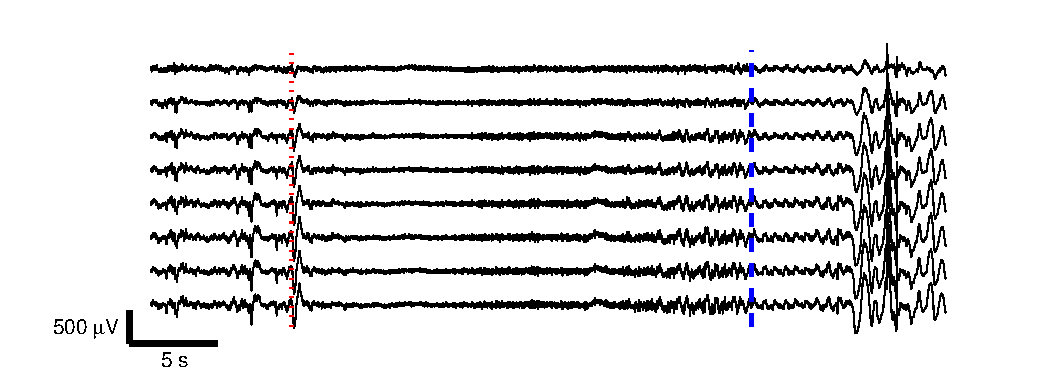
\includegraphics{./Figures/LFPs.eps}
\end{center}
\caption{{\bf Local field potentials from the micro-electrode array}. Data recorded from the first 8 channels of the array. The red dotted line indicates the seizure onset and the blue dashed line indicates the seizure end.}
\label{fig:TimeSeries}
\end{figure}


\begin{figure}[!ht]
\begin{center}
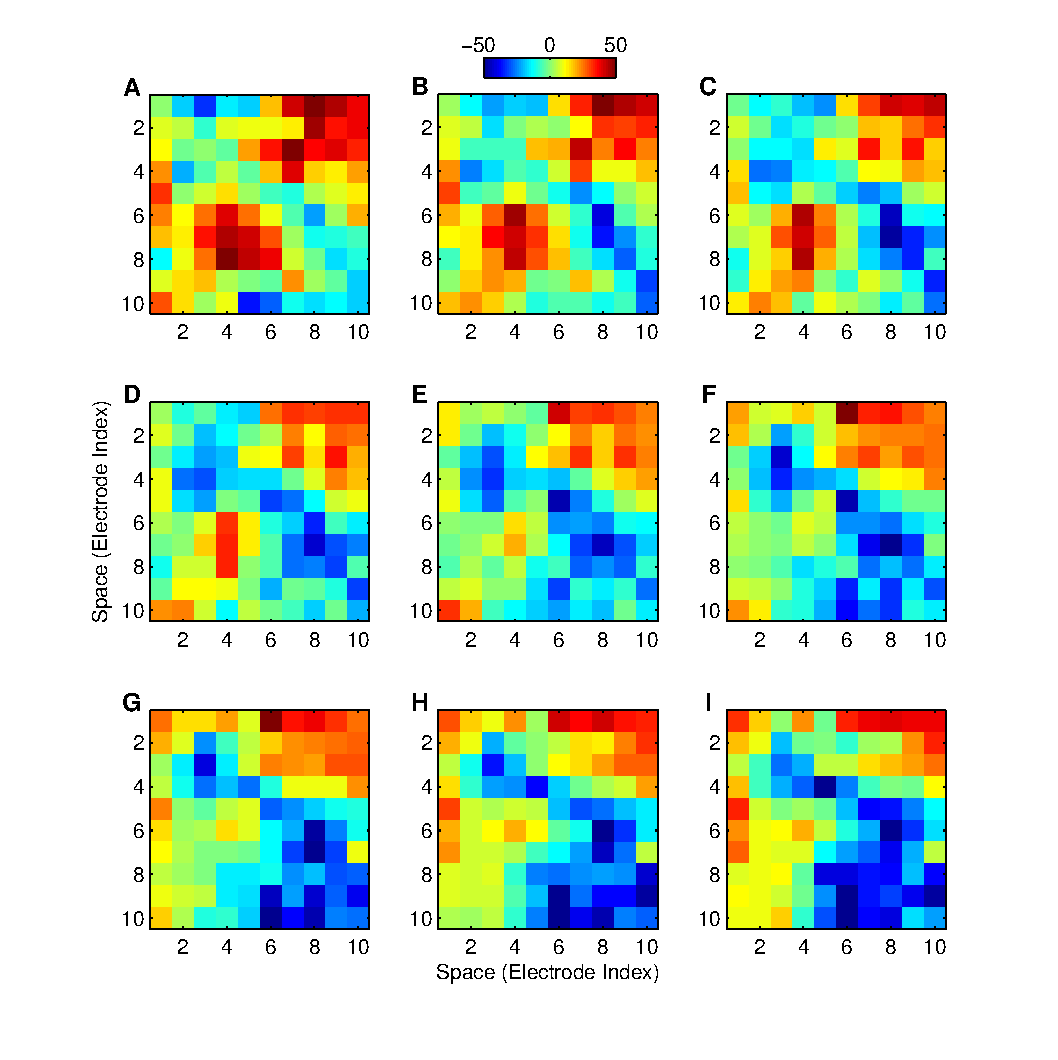
\includegraphics{./Figures/FieldObservations.eps}
\end{center}
\caption{{\bf Snap-shots of the spatial aspects of the observed field}. The snap-shots are ordered from A to I forming a consecutive sequence spaced 2.5~ms apart starting at 34.024s}
\label{fig:FieldObserations}
\end{figure}

\begin{figure}[!ht]
\begin{center}
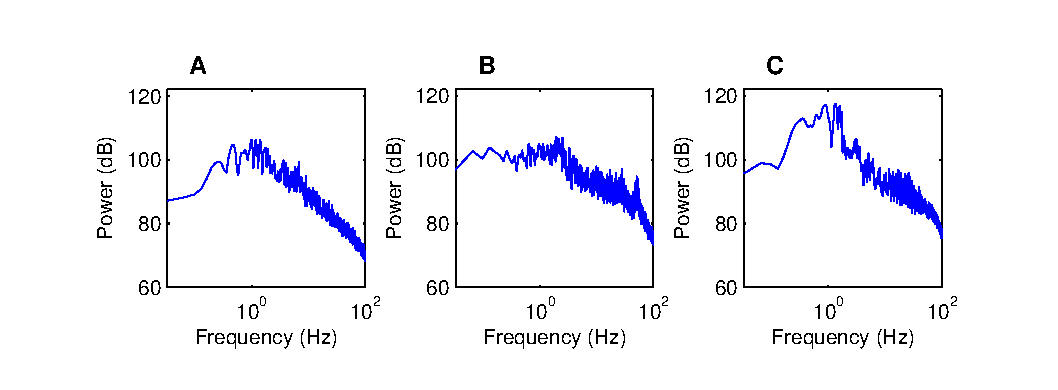
\includegraphics{./Figures/TemporalFreq.eps}
\end{center}
\caption{{\bf Spectra from local field potential recordings}. A. Pre-seizure observations. B. Seizure observations. C. Post-seizure observations.}
\label{fig:TemporalFreqObservation}
\end{figure}

\begin{figure}[!ht]
\begin{center}
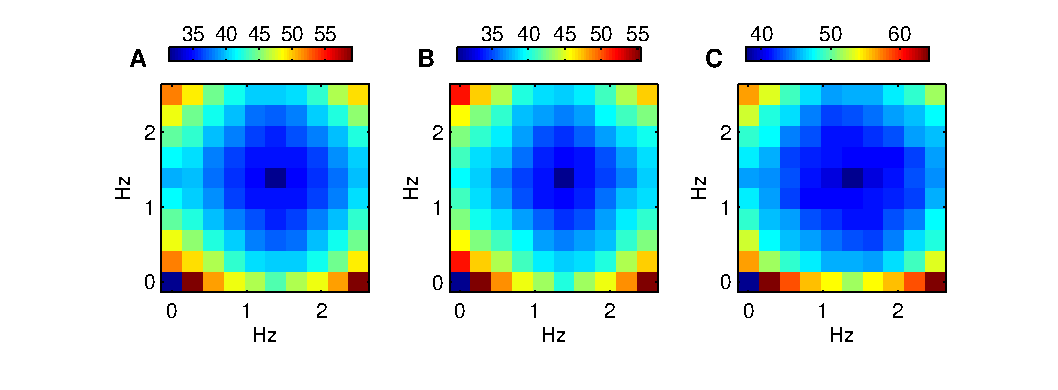
\includegraphics{./Figures/SpatialFreq.eps}
\end{center}
\caption{{\bf Spatial frequency analysis of the observed neural field}. A. Pre-seizure observations. B. Seizure observations. C. Post-seizure observations.}
\label{fig:SpatialFreqObservation}
\end{figure}

\begin{figure}[!ht]
\begin{center}
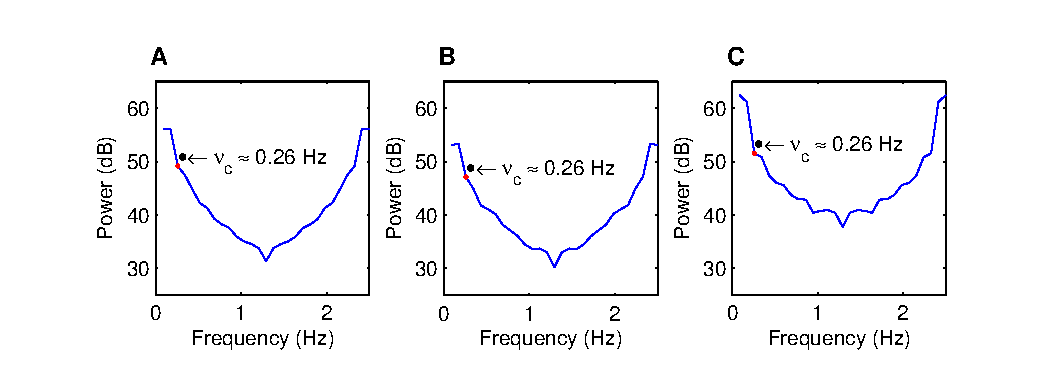
\includegraphics{./Figures/SpatialFreqCrossSection.eps}
\end{center}
\caption{{\bf Diagonal cross-section of the spatial frequency plots of the observed neural field}. A. Pre-seizure observations. B. Seizure observations. C. Post-seizure observations.}
\label{fig:DiagSpatialFreqObservation}
\end{figure}

\begin{figure}[!ht]
\begin{center}
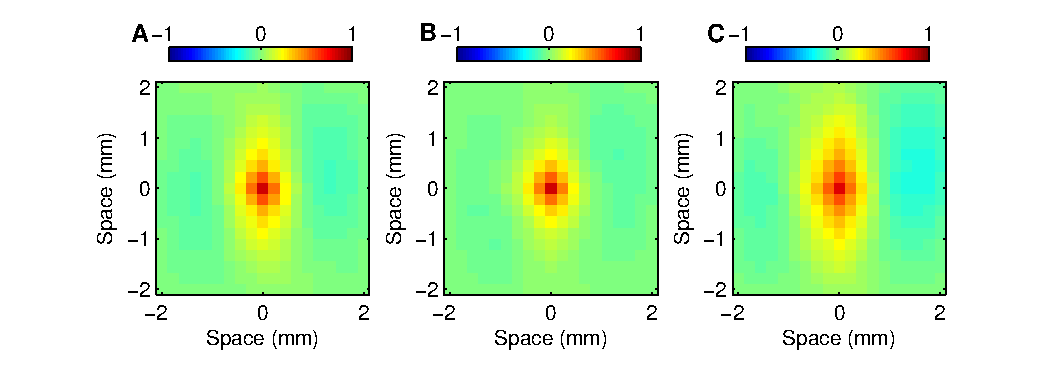
\includegraphics{./Figures/CrossCorr2D.eps}
\end{center}
\caption{{\bf Mean cross-correlations between consecutive observations of the neural field}. Note: The correlations are normalised such that the maximum value is one. A. Pre-seizure observation correlations. B. Seizure observation correlations. C. Post-seizure observation correlations.}
\label{fig:SpatialCrossCorrelation}
\end{figure}

\begin{figure}[!ht]
\begin{center}
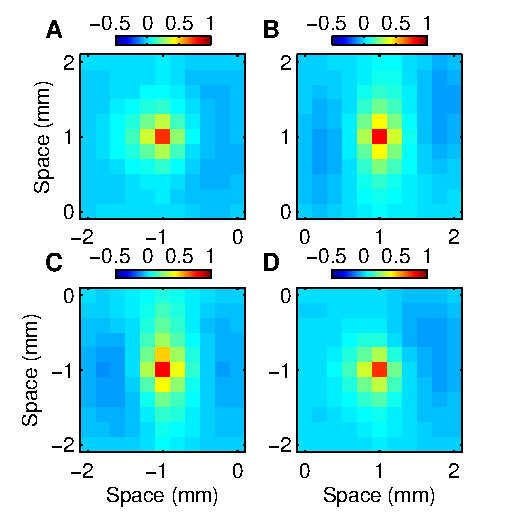
\includegraphics{./Figures/HomoTestCrossCorr.eps}
\end{center}
\caption{{\bf Mean cross-correlations between consecutive samples using subsets of observations of the neural field}. Each subplot shows correlations corresponding to a subset electrodes. Indexing the electrodes in a (x,y) grid, where index ranges from 1 to 10. Subplot A shows the mean correlation between electrode indexes (1-6, 5-10), subplot B shows correlations from indexes (5-10,5-10), subplot C shows indexes (1-6, 1-6) and subplot D shows indexes (5-10, 5-10).}
\label{fig:HomogeneityTest}
\end{figure}

% tables here
% ~~~~~~~~~~~
\renewcommand{\arraystretch}{1.7}
\begin{table}[!ht]
\caption{
\bf{Algorithm for the Unscented RTS Smoother}}
\begin{tabular}{|c|}\hline
\multicolumn{1}{|p{16cm}|}{\textbf{1.} Forward initialisation} \\ 
$\hat{\mathbf x}_0, \mathbf P_0$ \\
\hline
\multicolumn{1}{|p{16cm}|}{\textbf{2.} Forward iteration: for $t \in \left\lbrace 0,\cdots, T\right\rbrace $, calculate the sigma points $\mathcal X_{i,t}^f$ using equations \ref{eq:sigmapoints1}-\ref{eq:sigmapoints3} and propagate through equation~\ref{eq:QmatrixForSigmapoints}} \\
$\mathcal X_{i,t+1}^{f-}=Q(\mathcal X_{i,t}^f) \quad i=0, \dots, 2L$\\
\multicolumn{1}{|p{16cm}|}{Calculate the predicted state and the predicted covariance matrix} \\
$\hat{\mathbf x}_{t+1}^{f-}=\sum_{i=0}^{2L} W_i^{(m)}\mathcal X_{i,t+1}^{f-} $ \\
$\mathbf P_{t +1}^{f-}=\sum_{i=0}^{2L} W_i^{(c)}(\mathcal X_{i,t+1}^{f-}-\hat{\mathbf x}_{t +1}^{f-})(\mathcal X_{i,t+1}^{f-}-\hat{\mathbf x}_{t +1}^{f-})^\top+\boldsymbol \Sigma_e$ \\ 
\multicolumn{1}{|p{16cm}|}{Compute the filter gain, the filtered state and the filtered covariance matrix using the standard Kalman filter update equations} \\
$\mathcal K_{t+1}=\mathbf P_{t +1}^{f-}\mathbf C ^\top(\mathbf C \mathbf P_{t +1}^{f-}\mathbf C ^\top+\boldsymbol \Sigma_{\varepsilon})^{-1}$\\
$\hat{\mathbf x}_{t+1}^{f}=\hat{\mathbf x}_{t+1}^{f-}+\mathcal K_{t+1}(\mathbf y_{t+1}-\mathbf C\hat{\mathbf x}_{t +1}^{f-}) $\\
$\mathbf P_{t+1}^f=(\mathbf I - \mathcal K_{t+1}\mathbf C)\mathbf P_{t +1}^{f-}$\\ 
\hline
\multicolumn{1}{|p{16cm}|}{\textbf{3.} Backward initialisation}\\
$\mathbf P_T^b= \mathbf P_T^f, \quad \hat{\mathbf x}^b_T= \hat{\mathbf x}^f_T$ \\
\hline
\multicolumn{1}{|p{16cm}|}{\textbf{4.} Backward iteration: for $t \in \left\lbrace T-1, \cdots, 0 \right\rbrace $ calculate the sigma points $\mathcal X_{i,t}^b$ and propagate them through equation \ref{eq:QmatrixForSigmapoints}}\\
$\mathcal X_{i,t+1}^{b-}=Q(\mathcal X_{i,t}^b) \quad i=0, \dots, 2L$\\
\multicolumn{1}{|p{16cm}|}{Calculate the predicted state and the predicted covariance matrix}\\
$\hat{\mathbf x}_{t+1}^{b-}=\sum_{i=0}^{2L} W_i^{(m)}\mathcal X_{i,t+1}^{b-}$\\
$\mathbf P_{t +1}^{b-}=\sum_{i=0}^{2L} W_i^{(c)}(\mathcal X_{i,t+1}^{b-}-\hat{\mathbf x}_{t +1}^{b-})(\mathcal X_{i,t+1}^{b-}-\hat{\mathbf x}_{t +1}^{b-})^\top+\boldsymbol \Sigma_e $\\
$\mathbf M_{t +1}^{b-}=\sum_{i=0}^{2L} W_i^{(c)}(\mathcal X_{i,t}^{b-}-\hat{\mathbf x}_{t}^{f})(\mathcal X_{i,t+1}^{b-}-\hat{\mathbf x}_{t+1}^{b-})^\top$\\
\multicolumn{1}{|p{16cm}|}{Compute the smoother gain, the smoothed state and the smoothed covariance matrix}\\
$\mathbf S_t=\mathbf M_{t +1}^{b-}\left[ \mathbf P_{t +1}^{b-}\right] ^{-1} $\\
$\hat{\mathbf x}_t^b=\hat{\mathbf x}_t^f+\mathbf S_t\left[\hat{\mathbf x}_{t+1}^{b}-\hat{\mathbf x}_{t+1}^{b-}\right]$\\
$\mathbf P_{t}^{b}=\mathbf P_{t}^{f}+\mathbf S_t\left[\mathbf P_{t+1}^{b}-\mathbf P_{t+1}^{b-} \right]\mathbf S_t^\top $\\
\multicolumn{1}{|p{16cm}|}{Additional step to calculate the smoothed cross covariance matrix}\\
$\mathbf M_{t +1}^{b}=\mathbf S_t\mathbf P_{t+1}^{b}$\\
\hline
\end{tabular}
\begin{flushleft}This table shows the steps in the unscented Rauch-Tung-Striebel smoother algorithm. The steps are iterated 11 times for our state estimation procedure. The least squares algorithm is run after each iteration to update the parameter estimates.
\end{flushleft}
\label{tab:UKFAlgorithm}
\end{table}
\renewcommand{\arraystretch}{1}

\bibliographystyle{plain}
\bibliography{BrainIDE}
\end{document}
